\newpage
\subsection*{Question 1 -  Part A}

\noindent In the \verb|DemoTutorialTest| class, three methods are implemented, \verb|startBrowser()| and \verb|tearDown()| that respectively initiate and shutdown the driver in the browser, and \verb|demoTest()| that perfoms a test on a web browser window using the driver namely \textit{chromedriver}. In \verb|demoTest()|, there is first a waiting time, then the browser window is maximized, then the driver goes to google home page (\textit{https://www.google.\\com}), and finally, using the driver, we get the title of the page and assert that it must be equal to \textit{"Google"}.\\ It is worth noting that all the interactions with the browser during the test are done via \textit{chromedriver}, that has a multitude of tools to test user interface in a web browser environment. 

\begin{center}
        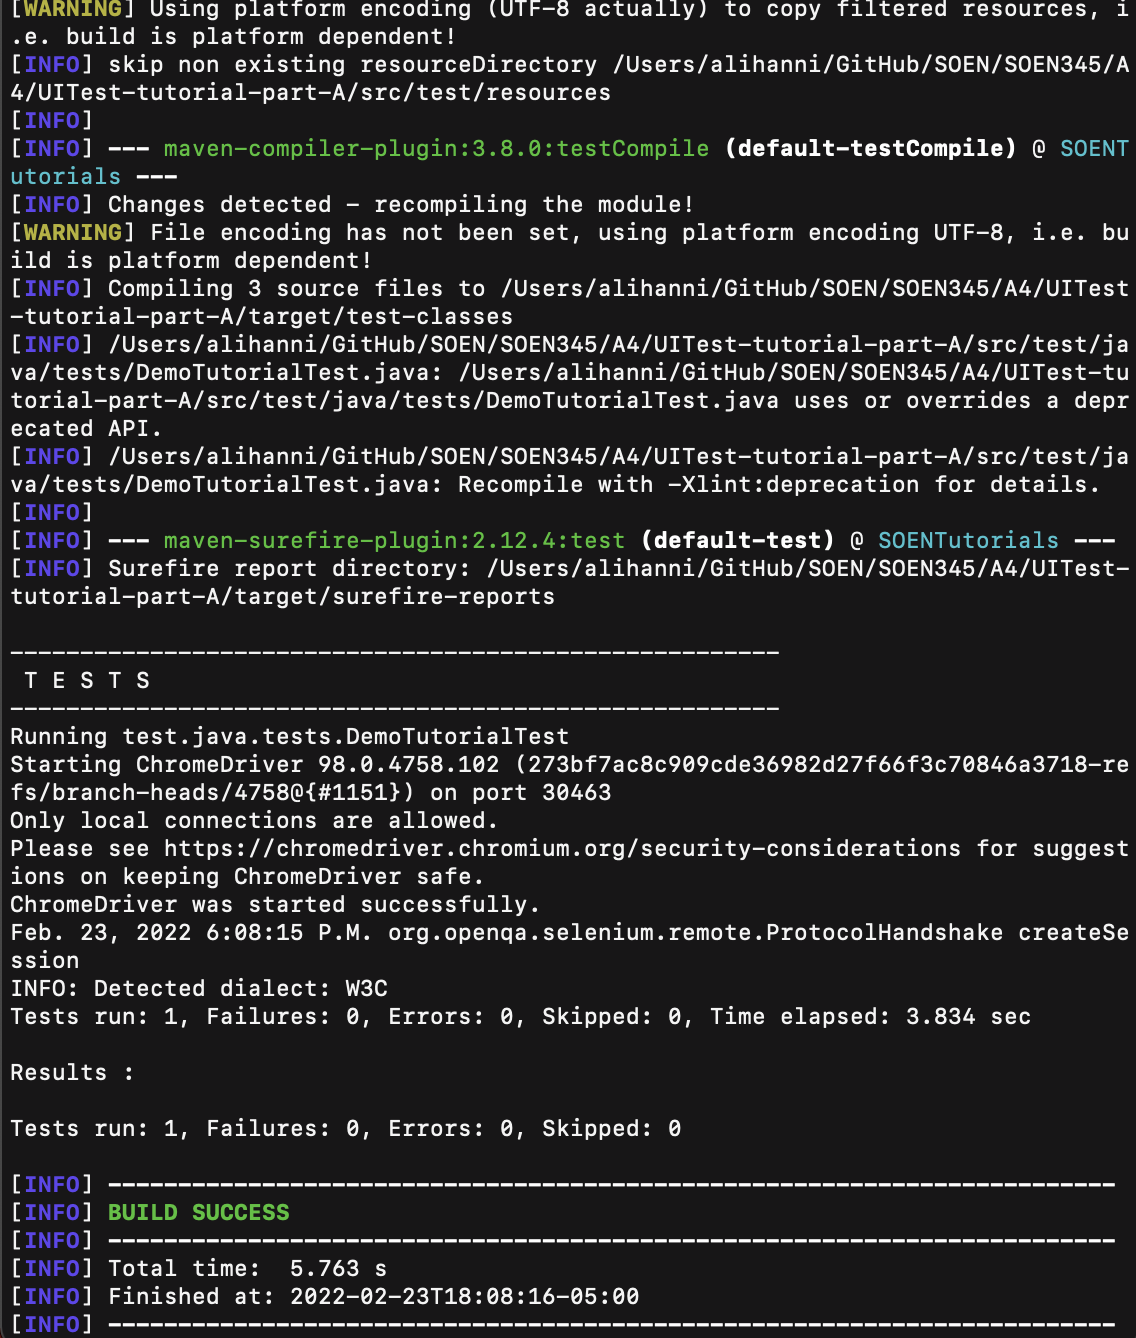
\includegraphics[width=0.85\textwidth]{img/partA.png}
        \noindent  \\The test has passed.
\end{center}
